\documentclass[t]{beamer}
\usepackage[utf8]{inputenc}
\usepackage[T1]{fontenc}
\usepackage{xcolor}
\usepackage{hyperref}
% \usepackage{enumitem}

\title{Bayesian data analysis with TensorFlow Probability}
\date{DataScienceConference Europe 2020}
\author{Simeon Carstens \& Dorran Howell, Tweag I/O}
\newcommand{\todo}{\textcolor{red}{\textbf{TODO}}}

\usetheme{Madrid}

\begin{document}

\begin{frame}
  \titlepage
\end{frame}


\begin{frame}
  \frametitle{Your hosts}
  \begin{block}{Simeon}
    \raisebox{-0.5\height}{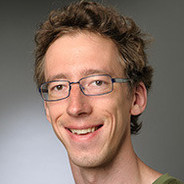
\includegraphics[width=0.15\paperwidth]{images/simeon}} ...will give the presentation \\
    \begin{itemize}
    \item background in computational structural biology
    \item Data Scientist at Tweag I/O since May 2019
    \end{itemize}
  \end{block}
  \begin{block}{Dorran}
    \raisebox{-0.5\height}{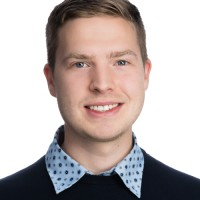
\includegraphics[width=0.15\paperwidth]{images/dorran}} ... will happily answers your questions in the chat\\
    \begin{itemize}
    \item background and previous positions in geophysics
    \item Data Scientist at Tweag I/O since August 2019
    \end{itemize}
  \end{block}
\end{frame}


\begin{frame}
  \frametitle{Tweag I/O}
  \todo \\
  Tweag I/O is a software innovation lab and consultancy based in Paris, but with employees all around the world.\\
  We specialize in
  \begin{itemize}
  \item software engineering, with a focus on functional programming
  \item DevOps, with a focus on reproducible software systems and builds
  \item data science
  \end{itemize}
\end{frame}


\begin{frame}
  \frametitle{What you're in for}
  This tutorial consists of alternating blocks of
  \begin{itemize}
  \item theory / example slides
  \item practical examples on either external websites or Google Colab notebooks. Links are provided at {\centering \url{https://github.com/tweag/tutorial-dsc-2020/}}
  \end{itemize}

  Requirements:
  \begin{itemize}
  \item a Google account (for the practical exercises)
  \item elementary knowledge in probability theory and statistics
  \end{itemize}
\end{frame}


\begin{frame}
  \frametitle{Bayesian vs frequentist probabilities}
  Example: fair coin flip with $p(\mathrm{head}) = p(\mathrm{tail}) = \frac{1}{2}$
  \begin{block}{Frequentist probability}
    \begin{description}
    \item[$p(\mathrm{"flip\ results\ in\ head"}|b=\frac{1}{2})=\frac{1}{2}$:] \hfill \\ $\frac{\mathrm{\# \ of \ heads}}{\mathrm{\# \ total \ flips}}$ for $\infty$ many fair coin flips
    \end{description}
  \end{block}
  \begin{block}{Bayesian probability}
    \begin{description}
    \item[$p(\mathrm{"flip\ results\ in\ head"}|b=\frac{1}{2})=\frac{1}{2}$:] \hfill \\ measure of \textit{belief} in the statement ``flip results in head'' given single fair coin flip
    \end{description}
  \end{block}
  \todo: this slide looks complicated and is aesthetically offputting
\end{frame}


\begin{frame}
  \frametitle{Prior beliefs}
  Assume: unknown bias $b$
  \begin{block}{Prior probability}
    Encodes prior belief in $b$ \textit{before} flipping the coin
  \end{block}
  What is known about $b$?
  \begin{itemize}
  \item $b$ is a probability: $0 \leq b \leq 1$
  \item most coins are fair
  \end{itemize}
  \begin{itemize}
  \item[$\rightarrow$] choose prior distribution defined between $0$ and $1$, with maximum at and symmetric around $b=\frac{1}{2}$
  \end{itemize}
  Example:
  \begin{equation*}
    b \sim \mathrm{Beta}(\alpha=2,\beta=2)
  \end{equation*}
  with
  \begin{equation*}
    \mathrm{Beta}(x|\alpha, \beta) \propto x^{\alpha-1}(1-x)^{\beta-1}
  \end{equation*}
\end{frame}


\begin{frame}
  \frametitle{Posterior belief}
  Now: flip coin one time, result: $\mathrm{head}$
  \begin{block}{Posterior belief}
    \begin{description}
      \item[$p(b|\mathrm{head})$:] updated prior belief after obtaining new data
    \end{description}
  \end{block}
  \todo: some illustration of shifting distribution
\end{frame}


\begin{frame}
  \frametitle{Update rule}
  \begin{block}{Bayes' theorem}
    \begin{equation*}
      p(A|B) = \frac{p(B|A) \times p(A)}{p(B)}
    \end{equation*}
    (easily derived from rules for conditional probabilities)
  \end{block}
  In data analysis:
  \begin{equation*}
    \underbrace{p(x|D,I)}_{\mathrm{posterior}} = \underbrace{p(D|x,I)}_{\mathrm{likelihood}} \times \underbrace{p(x|I)}_{\mathrm{prior}} / \underbrace{p(D|I)}_{\mathrm{evidence}}
  \end{equation*}
  \begin{description}
  \item[$x$:] model parameter
  \item[$D$:] data
  \item[$I$:] prior information (often not made explicit)
  \end{description}
\end{frame}


\begin{frame}
  \frametitle{Update rule}
  In our coin flip example:
  \begin{description}
  \item[prior:] $p(b) \propto b^\frac{1}{2} (1-b)^\frac{1}{2}$
  \item[likelihood]: $D \sim \mathrm{Bernoulli}(b)$, thus:
    \begin{equation*}
      bla
    \end{equation*}
  \end{description}
\end{frame}

\end{document}